\documentclass[a4paper, 11pt, titlepage]{article}
\usepackage{graphicx}
\usepackage{pdfpages}
\usepackage{fancybox}
\usepackage[francais]{babel}
\usepackage[utf8]{inputenc}
% \usepackage[T1]{fontenc}
\usepackage{amsmath,amsfonts,amssymb}
\usepackage{fancyhdr}
\usepackage{stackrel}
\usepackage{babel,indentfirst}
\usepackage{xspace}
\usepackage{url}
\usepackage{titling}
\usepackage{listings}
\usepackage{color}
\usepackage{array}
\usepackage{hyperref}
\usepackage{makecell}
\usepackage{tikz}
\usepackage{float}
\usepackage{wrapfig}

%\setlength{\parindent}{0pt}
\setlength{\parskip}{1ex}
\setlength{\textwidth}{17cm}
\setlength{\textheight}{24cm}
\setlength{\oddsidemargin}{-.7cm}
\setlength{\evensidemargin}{-.7cm}
\setlength{\topmargin}{-.5in}


\lstset{
  sensitive=f,
  morestring=[d]",
  showstringspaces=false,
  basicstyle=\small\ttfamily,
  keywordstyle=\bf\small,
  commentstyle=\itshape,
  stringstyle=\sf,
  extendedchars=true,
  columns=[c]fixed
}



\predate{
\begin{center}
}
\postdate{
\\
\vspace{1.5cm}

\includegraphics[scale=0.7]{imag.png}
\end{center}}


\title {{ {\huge Manuel utilisateur de la stack SMACK }} }

\author{%\Large Equipe ?? \\
%\\
    {\sc Ait El Kadi}~Ouiame,
    {\sc Ansari}~Othmane,
    {\sc Boudouin}~Philippe,\\
    {\sc Boukrouh}~Insaf,
    {\sc Giroux}~Baptiste,
    {\sc Gouttefarde}~Léo,\\
    {\sc Kodjo}~Edoh,
    {\sc Nahyl}~Othmane
}

\date{Mardi 24 Janvier 2017}

\lhead{Stack SMACK}
\rhead{Manuel utilisateur}

\begin{document}
\pagestyle{fancy}
\maketitle

\setcounter{tocdepth}{2}

\tableofcontents
\newpage


\section {Mise en route}

Pour commencer rapidement, un fichier \href{https://github.com/leogouttefarde/smack/blob/master/README.md}{README.md} décrivant les éléments essentiels est fourni.


\section {Installation / désinstallation}

\subsection {Première installation}

Avant l'installation initiale de la stack sur le cluster, il faut lancer la commande suivante :

\begin{verbatim}
ZIP=~/setup.zip; cd ~; wget -O $ZIP \
  https://raw.githubusercontent.com/leogouttefarde/smack/master/setup.zip; \
  sudo apt -y install unzip; unzip -o $ZIP
\end{verbatim}

Une fois la stack installée, les scripts de gestion deviennent disponibles sur l'ensemble des machines du cluster.


\subsection {Installation}

Pour lancer l'installation de la stack, il suffit de lancer le script \lstinline!~/scripts/install_all.sh!


\subsection {Désinstallation}

Pour désinstaller la stack, il faut lancer le script \lstinline!~/scripts/uninstall_all.sh!


\subsection {Mise à jour des scripts}

Pour mettre à jour les scripts, il suffit de lancer le script \lstinline!~/scripts/update_setup.sh!



\section {Gestion du cycle de vie}

\subsection {Démarrage}

\subsubsection*{run\_cassandra\_cluster.sh}
Permet de lancer les processus Cassandra sur tous les noeuds du cluster en appellant \lstinline!run_cassandra_local.sh! sur chaque noeud.
Le script inverse est \lstinline!stop_cassandra_cluster.sh! .

\subsubsection*{run\_cassandra\_local.sh}
Permet de lancer les processus Cassandra sur un hôte, il détecte aussi l'état du noeud Cassandra pour décider de la manière du lancement (start normal ou remplacement).
Le script inverse est \lstinline!kill_mesos_processes.sh! .

\subsubsection*{run\_kafka\_cluster.sh}
Permet de lancer le scheduler kafka et de démarrer les brokers. Le nombre de ceux-ci est passé en argument.
Le script inverse est \lstinline!stop_kafka_cluster.sh! .

\subsubsection*{run\_mesos\_cluster.sh}
Permet de démarrer le cluster mesos sur tous les maîtres et esclaves du cluster.
Le script inverse est \lstinline!stop_mesos_cluster.sh! .

\subsubsection*{run\_mesos\_local.sh}
Permet de démarrer les daemons mesos. La commande de démarrage est différente selon le type de l'hôte.
Le script inverse est \lstinline!kill_mesos_processes.sh! .



\subsection {Arrêt}

\subsubsection*{stop\_cassandra\_cluster.sh}
Arrête le cluster Cassandra.


\subsubsection*{stop\_kafka\_cluster.sh}
Arrête le cluster Kafka.


\subsubsection*{stop\_mesos\_cluster.sh}
Arrête le cluster Mesos.


\subsubsection*{kill\_cassandra\_processes.sh}

Tue les processus Cassandra localement.


\subsubsection*{kill\_cassandra\_server.sh}

Tue les processus Cassandra sur le serveur fourni en paramètre.


\subsubsection*{kill\_mesos\_server.sh}

Tue les processus Mesos sur le serveur fourni en paramètre.


\subsubsection*{kill\_mesos\_processes.sh}

Tue les processus Mesos localement.


\subsubsection*{kill\_kafka\_broker.sh}

Tue le brokers Kafka de numéro fourni en paramètre.



\subsection {Utilitaires}

\subsubsection*{cassandra\_status.sh}

Affiche l'état du cluster Cassandra.


\subsubsection*{install\_hosts.sh}
Permet de configurer le fichier \lstinline!/etc/hosts! sur toutes les machines en appellant le script \lstinline!declare_hosts.sh! sur chacune de celles-ci.
Le script inverse est \lstinline!uninstall_hosts.sh! .


\subsubsection*{update\_setup.sh}

Met à jour les différents scripts sur tous les noeuds du cluster.


\subsubsection*{declare\_hosts.sh}

Permet de configurer, ou de rétablir l'ancienne configuration des hôtes en cas de désinstallation.


\subsubsection*{version.sh}

Affiche le hash MD5 de l'archive actuellement installée.


\subsubsection*{run\_cmd\_all.sh}

Lance la commande fourni en paramètre sur tous les noeuds.



\section {Supervision du cluster}
\subsection{M/Monit}

L'interface M/Monit permet de superviser l'état du cluster depuis le port 8080 de chaque machine, qui fournit une interface web dédiée.

Depuis cette interface, il est possible d'observer le cluster et de voir si un service est en panne par exemple.
Si c'est le cas, le service est automatiquement redémarré sous 2 minutes maximum.

Il est également possible de forcer le démarrage d'un service, l'arrêter, le redémarrer ou lancer un monitoring de service manuellement au lieu d'attendre.

Aussi, il possible d'effectuer différentes statistiques sur le cluster et de consulter le journal des événements.


\subsection{Mesos}

Mesos fournit lui aussi une interface Web pratique pour la supervision de l'état du cluster Mesos, accessible depuis le port 5050 par défaut sur chacun des masters.

\begin{figure}[H]
    \centering
    \centerline{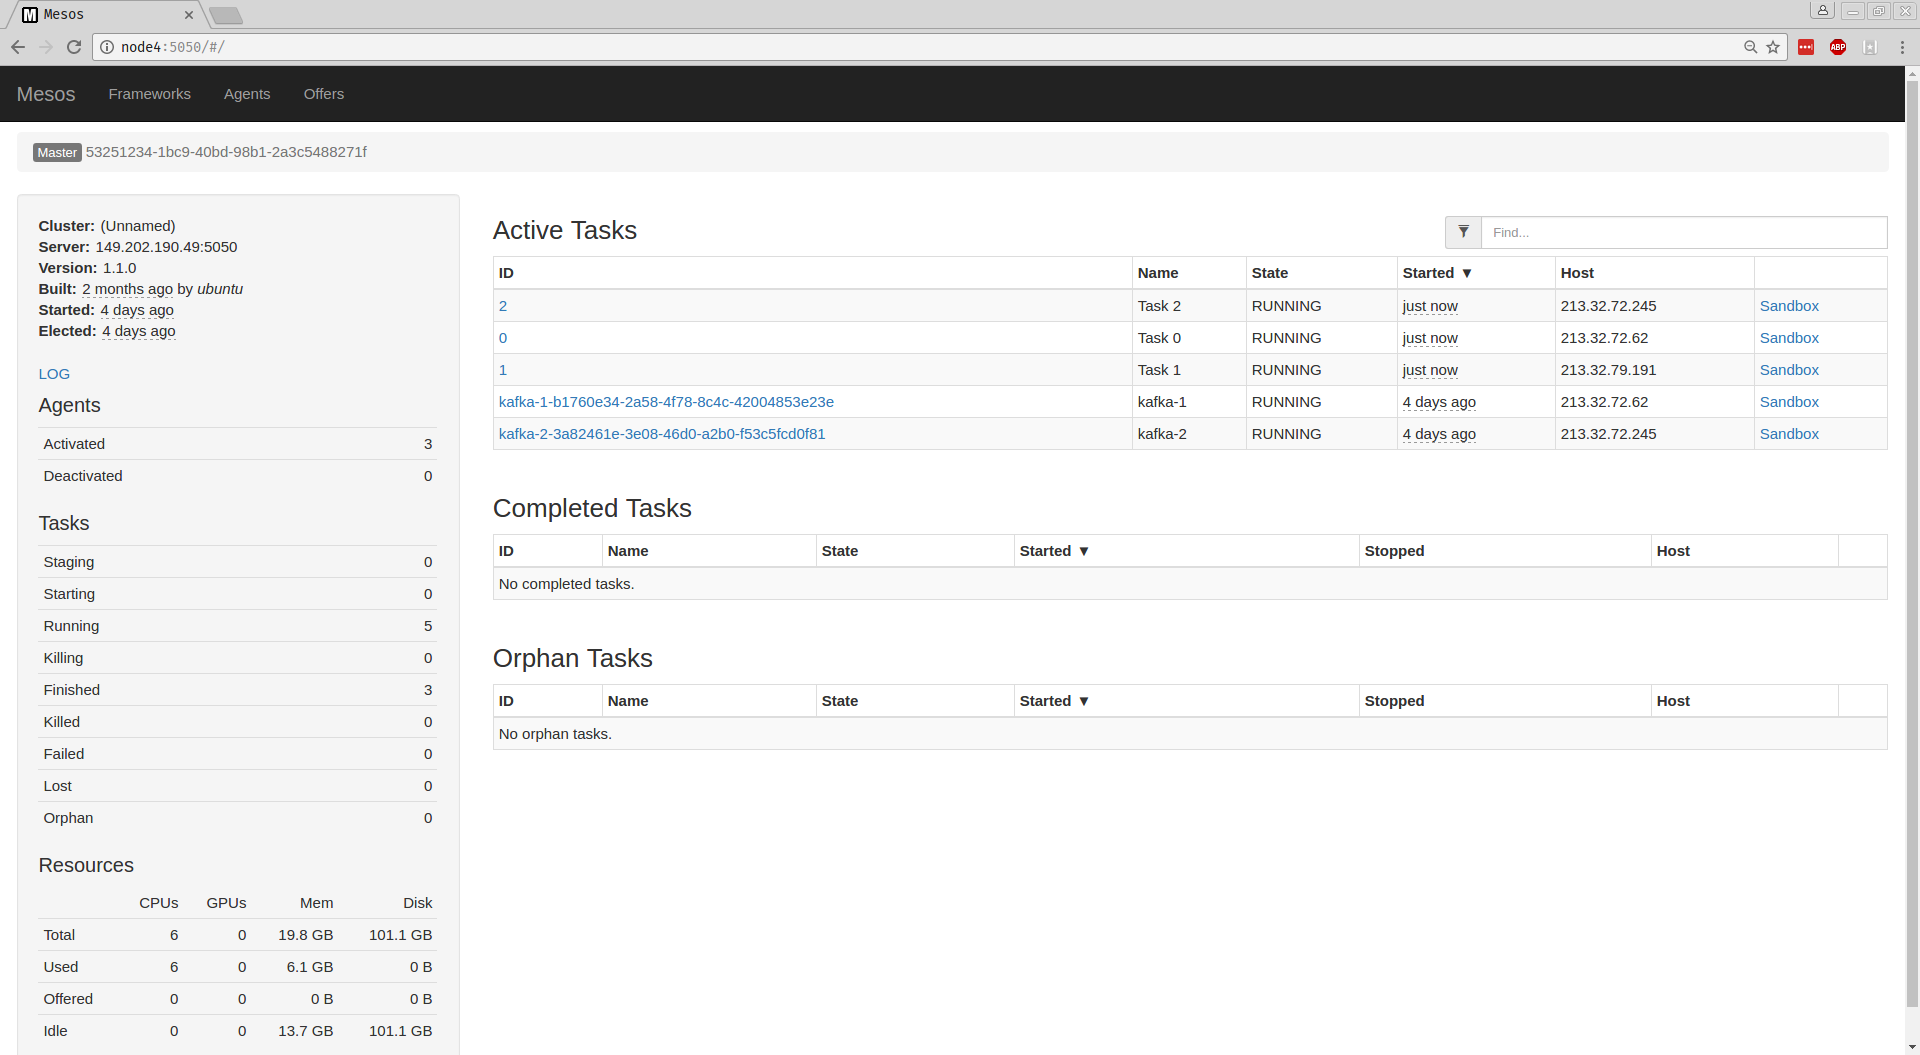
\includegraphics[scale=0.23]{res/mesos.png}}
    \caption{Web UI d'accueil de Mesos}
\end{figure}
Comme on peut le voir, l'interface fournit des informations utiles sur l'utilisation des ressources des différents agents du cluster. Elle donne également une vue globale sur les différentes tâches en cours déployées sur le cluster. \\Lorsqu'on clique sur le bouton "Frameworks" au niveau de la barre de navigation, on obtient une interface contenant plus de détails sur les frameworks déployés sur les noeuds.
\begin{figure}[H]
    \centering
    \centerline{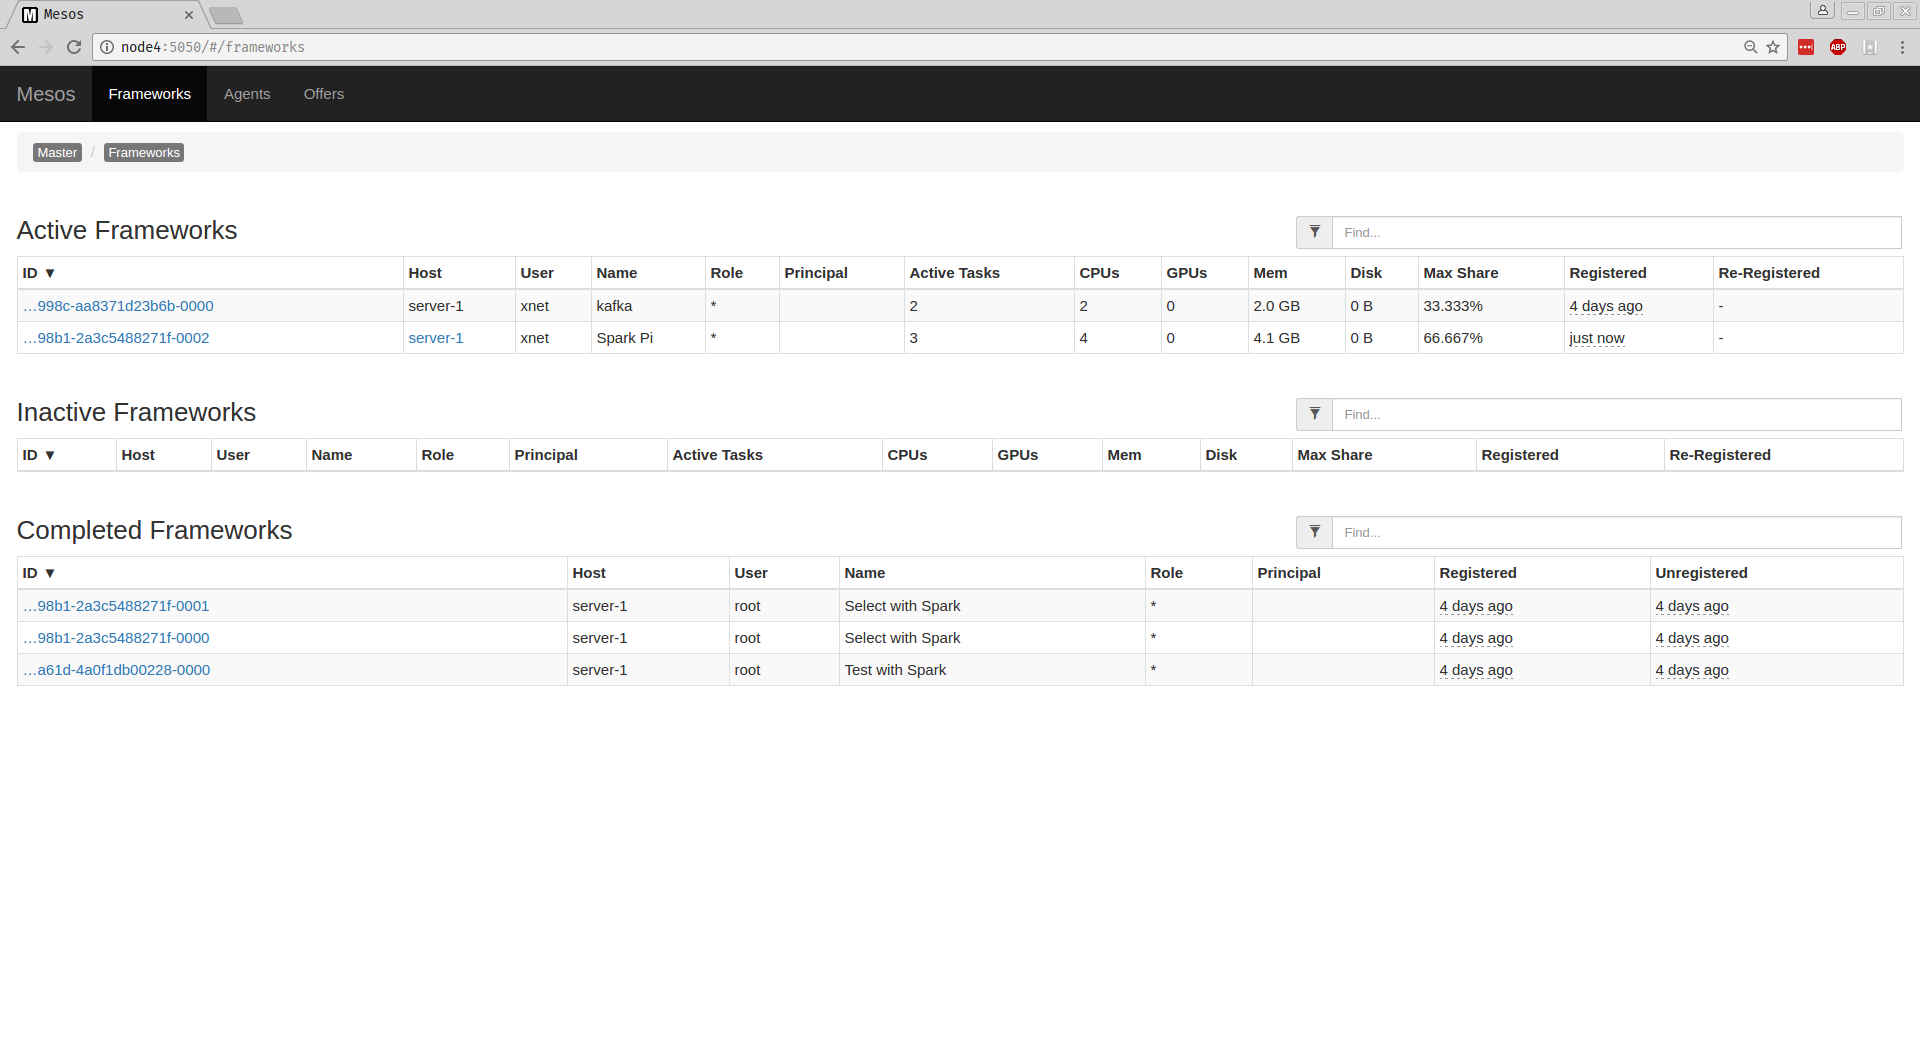
\includegraphics[scale=0.23]{res/fra.png}}
    \caption{Vue détaillée des frameworks en cours}
\end{figure}
Dans cet exemple-ci, un job spark est lancé. On peut cliquer sur le lien du framework pour obtenir des détails les exécuteurs du jobs.\\


\begin{figure}[H]
    \centering
    \centerline{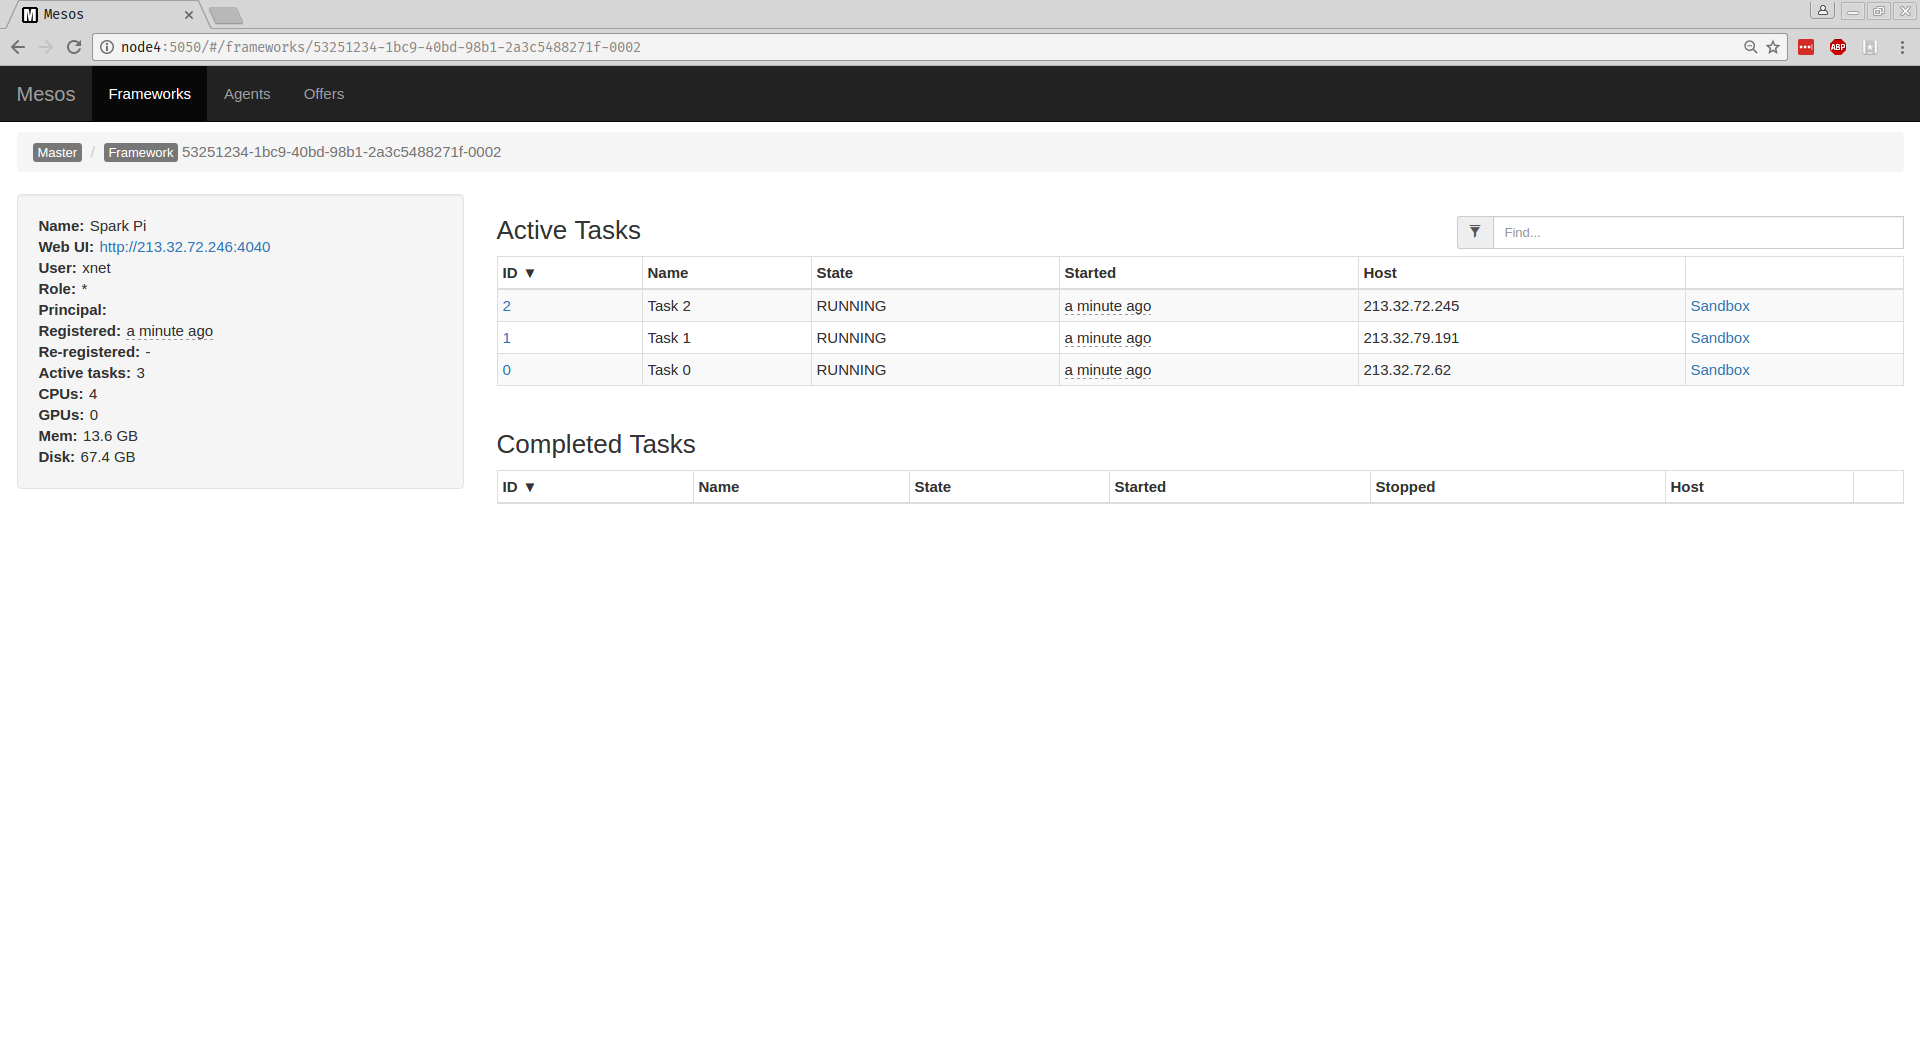
\includegraphics[scale=0.23]{res/tasks.png}}
    \caption{Vue détaillées sur les taches d'un framework}
\end{figure}
Quand on clique sur l'url du Web UI visible sur la barre gauche de la page, on accède à l'interface web de spark valable pour toute la durée du job.
\newpage
\subsection{Spark}
L'interface d'accueil donne une vue générale sur tous les jobs en cours et leur état d'avancement.
\begin{figure}[H]
    \centering
    \centerline{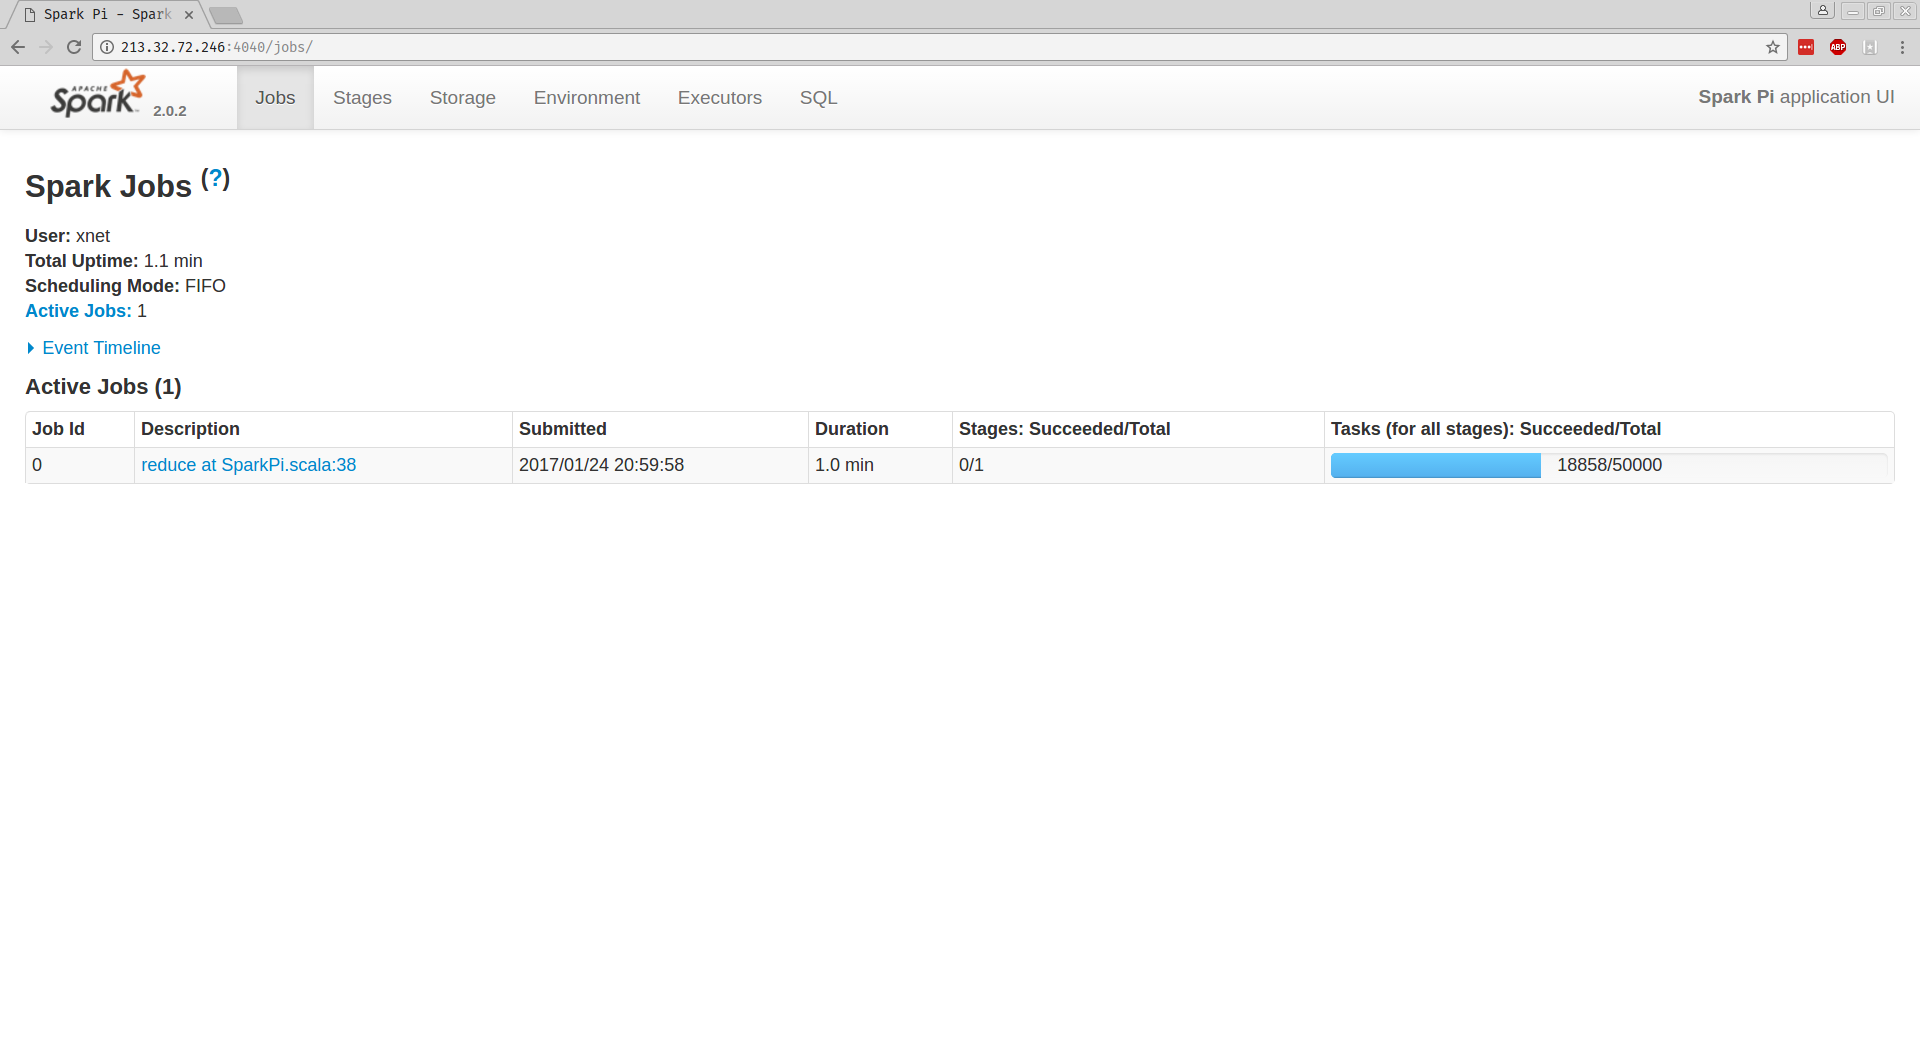
\includegraphics[scale=0.23]{res/sphome.png}}
    \caption{Vue générale des différents jobs Spark}
\end{figure}
On peut choisir de voir encore plus de détails sur les étapes internes du job. On a également accès au DAG du job, qui en est une représentation en graphe direct acyclique.\\


\begin{figure}[H]
    \centering
    \centerline{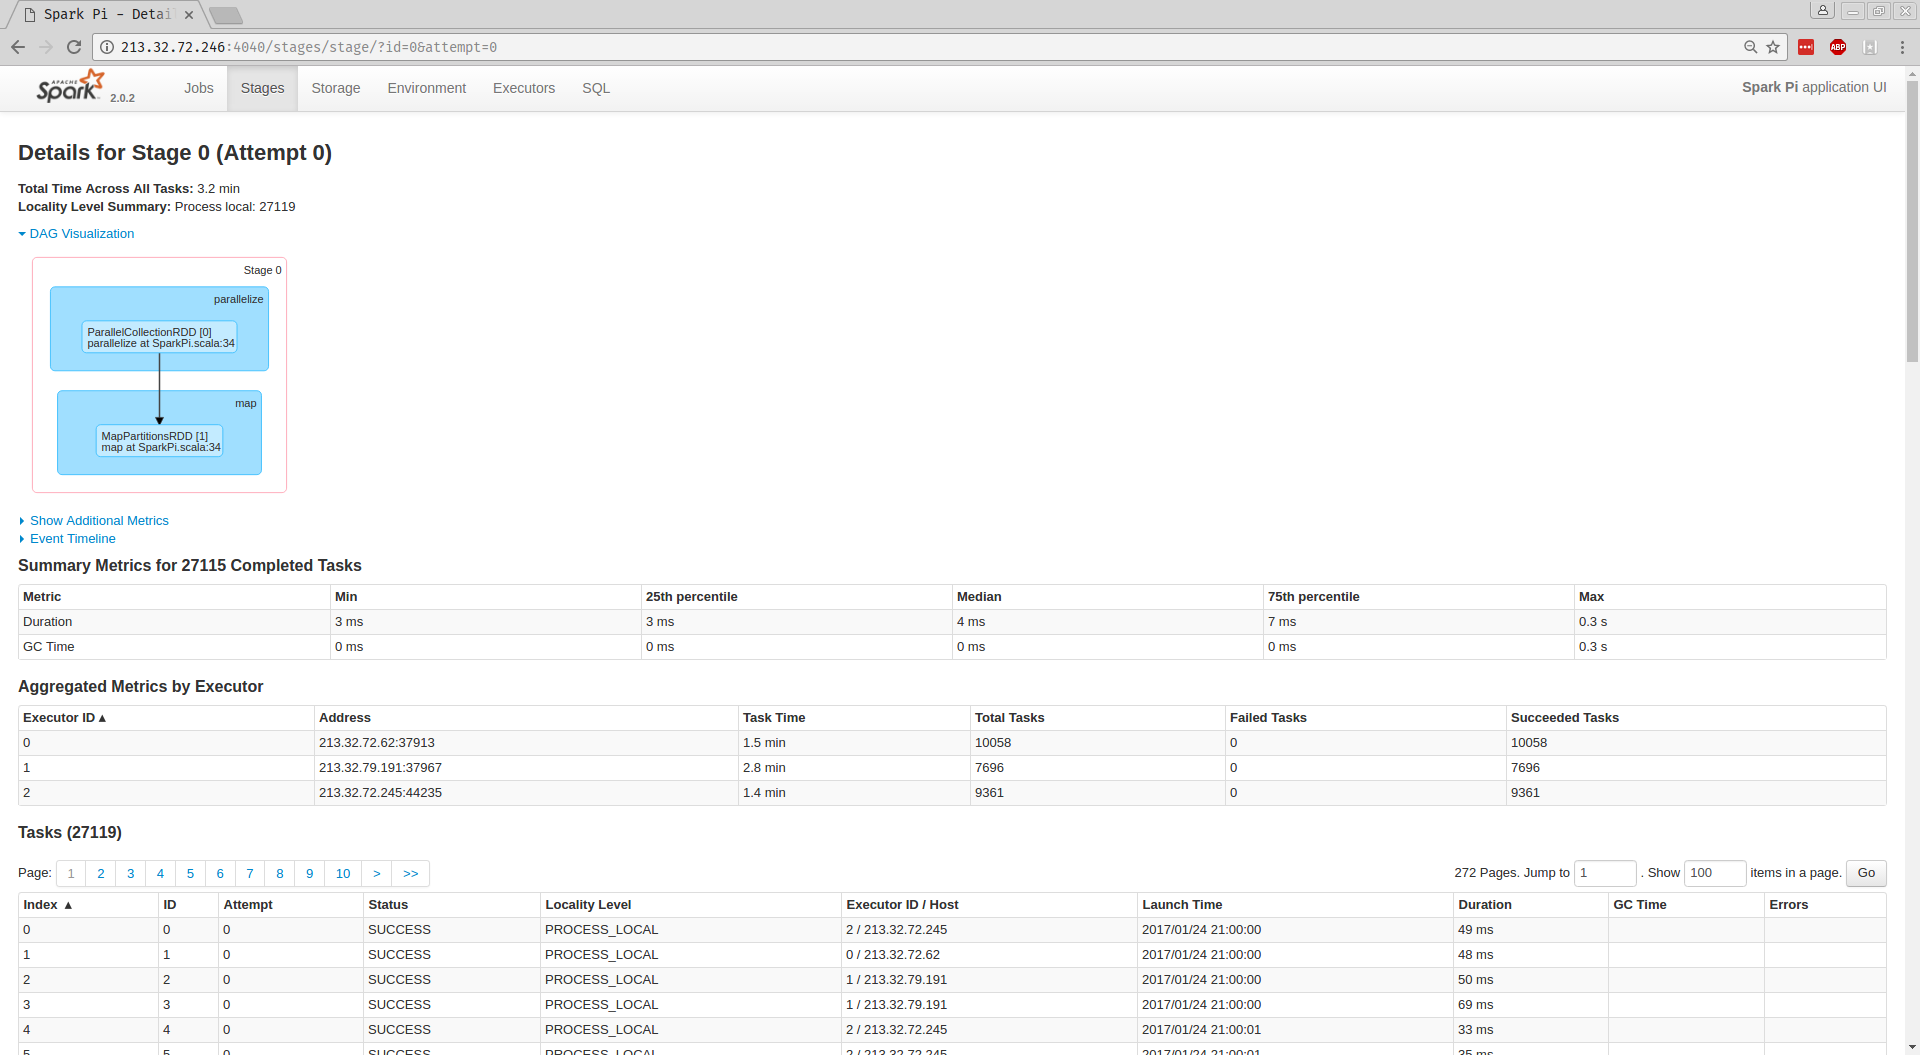
\includegraphics[scale=0.23]{res/jobdetails.png}}
    \caption{Vue détaillée d'un job Spark}
\end{figure}


\newpage

\section {Application de démonstration}

Pour le développement de l'application de démonstration, nous avons utilisé le langage de programmation Scala.

L'application concerne un dataset qui contient des données sur les voyages des taxis de NYC en date de 2013, et dont les champs sont les suivants :

\noindent medallion, hack\_license, vendor\_id, pickup\_datetime, payment\_type, fare\_amount, surcharge, mta\_tax, tip\_amount, tolls\_amount, total\_amount

$\newline$
L'application peut être décomposée en deux parties :

\subsection {L'intégration de données}

\begin{center}
% \begin{figure}[ht!]
    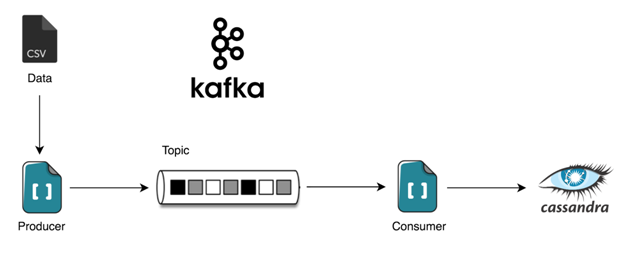
\includegraphics[scale=0.55]{res/demo1.png}
% \caption{Diagramme des cas d'utilisation}
% \end{figure}
\end{center}

Le producteur Kafka est un programme Scala qui permet de lire un fichier CSV à l'aide d'un itérateur (puisque le fichier est très volumineux et ne peut pas être chargé complètement en une seule fois). Chaque ligne lue est par la suite envoyée à un broker Kafka. Pour exécuter un programme Scala, il suffit de taper la commande "scala + nom du fichier".

Le consommateur Kafka est un programme écrit en Scala et exécuté avec Spark. Pour exécuter un programme en Spark, on aura besoin de produire un fichier jar relatif au programme à l'aide de SBT.  La communication entre le producteur et le consommateur se fait au moyen de topic qui permet de séparer les catégories de données. Dans notre architecture, nous n'avons utilisé qu'un seul topic pour garantir le flux de communication entre le producteur Kafka et le consumer Kafka.

Pour ceci, on met le programme dans un dossier main qui lui même est contenu dans un dossier src, ensuite, à la racine du projet, on crée un fichier SBT qui contient toutes les dépendances dont on aura besoin lors de la compilation du programme (dépendances de Kafka, Cassandra, etc.) avec leurs versions spécifiées. La commande "sbt package" permet alors de générer ce jar, qui sera exécuté ensuite avec spark-submit (le connecteur de Cassandra est spécifié après --packages, et les jars externes après --jars et séparés par des virgules).

Chaque 40ms, le consommateur "consulte" le broker Kafka pour voir s'il y'a des lignes à "consommer" (un offset l'aide à savoir où il en est). Les lignes du fichier des données sont ensuite converties en dataframes et insérées dans la base de données Cassandra (qui a été créée au début).
 

\subsection {Le traitement des données}

\begin{center}
% \begin{figure}[ht!]
    
\includegraphics[scale=0.55]{res/demo2.png}
% \caption{Diagramme des cas d'utilisation}
% \end{figure}
\end{center}

La partie "Traitement" consiste en un programme Spark écrit en Scala, sa compilation et son exécution sont les mêmes que le consommateur (avec la seule différence qu'on aura pas besoin des jars externes).

Le programme lit les données de Cassandra et les met dans des dataframes. Ces dataframes pourront êtres mis dans des tables temporaires pour pouvoir effectuer des requêtes SQL brutes, ou bien on peut en effectuer des transformations Spark directement comme map, flatmap, groupby, etc.
Les résultats des traitements sont stockées dans d'autres tables de notre base de données Cassandra.\\


On propose plusieurs types de traitement, par exemple :

\begin{itemize}
\item
Nombre de transactions et chiffre d'affaire pour chaque méthode de paiement.
\item
Chiffre d'affaire pour chaque vendeur.
\item
Nombre de transactions pour chaque type de voyage.\\
\end{itemize}


Remarques :

\begin{itemize}

\item
Les brokers de Kafka doivent être indiqués dans les deux premiers programmes (pour l'écriture et la lecture).

\item
Dans Cassandra, on a 2 datacenters avec une stratégie de réplication “Network Topology Strategy” et  un degré de 3
 
\end{itemize}




\end{document}


